\label{sec:exp}
%In this section we systematically evaluate our system.

%As no one else has attempted to predict 3D point clouds by networks, we first justify the advantage of this representation over commonly used ones for deep learning systems. To this end we compare with the state-of-the-art volume based approach on the task of 3D reconstruction from a single RGB image (Sec~\ref{sec:exp:rgb}). In addition, we evaluate our system's ability on 3D shape completion, to check how well it captures and uses object structure cues such as symmetry (Sec~\ref{sec:exp:depth}). % We further compare the performance of our models with human, to get a sense how challenge these tasks are. (Sec~\ref{sec:exp:human})

%Different from existing 3D reconstruction network that only predicts a single output, our method is a conditional sampler. We examine its sampling ability in Sec~\ref{sec:exp:gan}.

%Since the design of point set prediction network is completely novel, we conduct various analysis experiments to validate the effectiveness of main design choices, focusing on network architecture and loss function (Sec~\ref{sec:exp:analysis}).



\begin{figure}[t!]
  \centering
  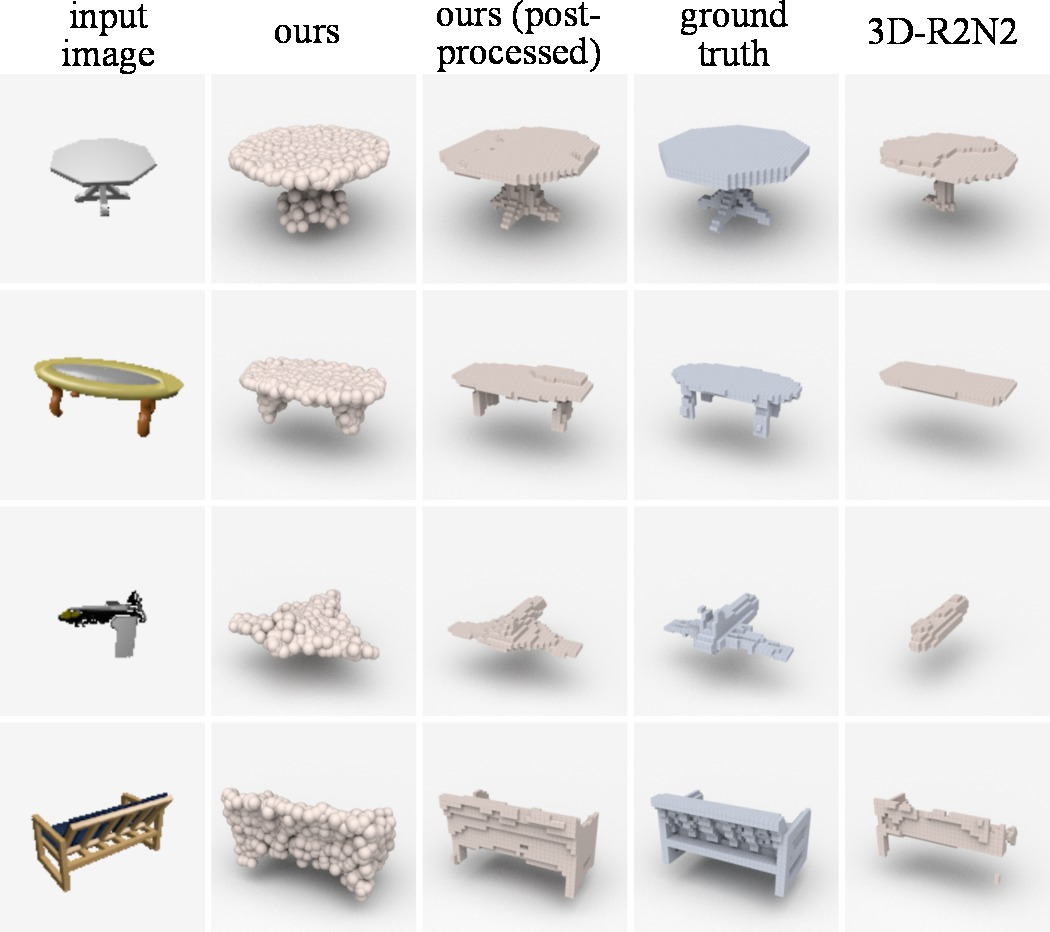
\includegraphics[width=\linewidth]{./fig/show_r2n2}
  \caption{Visual comparison to 3D-R2N2. Our method better preserves thin structures of the objects. }\label{fig:visual_comparison}
\end{figure}

\subsection{Training Data Generation by Synthesis}
\label{sec:exp:traindata}
To start, we introduce our training data preparation. We take the approach of rendering 2D views from CAD object models. % The models can be retrieved from on-line 3D repositories (e.g. Google Warehouse) in large volume. 
Our models are from the ShapeNet dataset~\cite{shapenet2015}, containing large volume of manually cleaned 3D object models with textures. Concretely we used a subset of 220K models covering 2,000 object categories. The use of synthesized data has been adopted in a number of existing works~\cite{choy20163d,rezende2016unsupervised}.

\begin{figure}[t!]
  \centering
  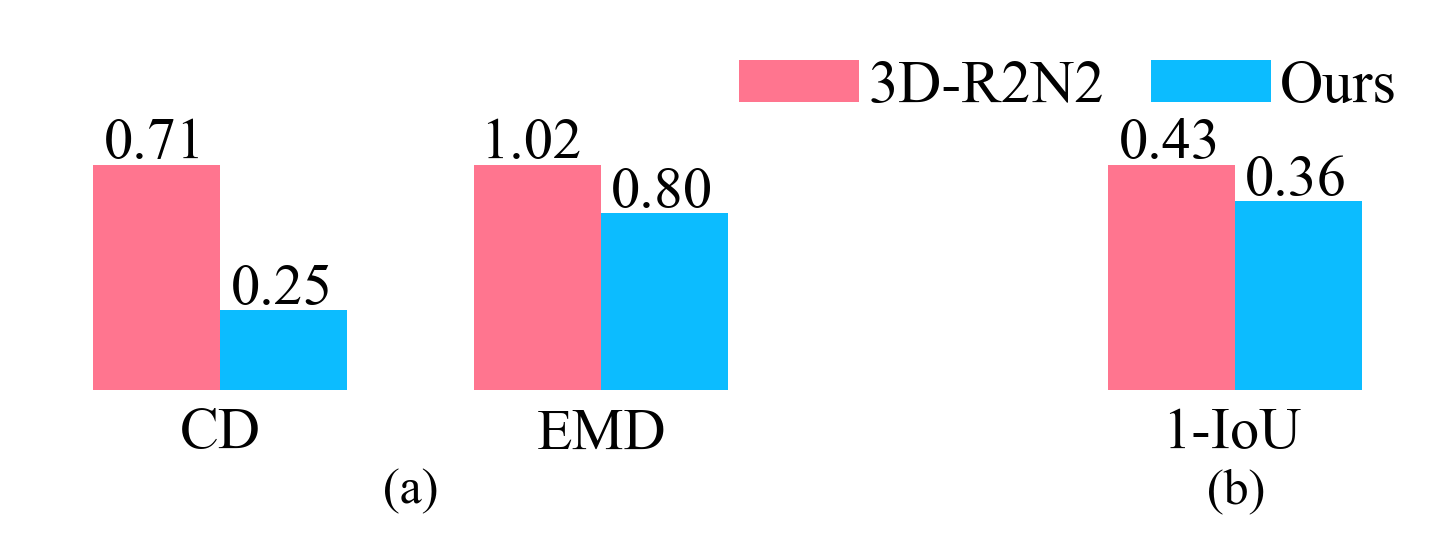
\includegraphics[width=0.9\linewidth]{./fig/iou_bar}
  \caption{Quantitative comparison to 3D-R2N2. (a) Point-set based metrics CD and EMD. (b) Volumetric representation based metric 1 - IoU. Lower bars indicate smaller errors. Our method gives better results on all three metrics. }\label{fig:comparison}
\end{figure}
For each model, we normalized the radius of its bounding hemi-sphere to unit $1$ and aligned their ground plane. Then each model was rendered into 2D images according to the Blinn-Phong shading formula with randomly chosen environmental maps. In our experiments we used a simple local lightening model for the sake of computation time. However, it is straight-forward to extend our method to incorporate global illumination algorithms and more complex backgrounds. % The bounding hemi-sphere is preferred to sphere so that we can place the model on a ground plane.

% \hao{i have a question here. we should discuss.} As for the relative camera pose, we considered two settings in our experiment. In the \textbf{studio} setup, images are taken from a fixed elevation angle. This is justifiable as images are commonly accompanied by gyroscopic information when they are captured (e.g. in a smart-phone or a human's head). In the \textbf{free-view} setup, we used randomized elevation and azimuth angles to better fit the distribution of uncontrolled Web images.

\subsection{3D Shape Reconstruction from RGB Images}


\label{sec:exp:rgb}
\paragraph{Comparison to state-of-the-art}
We compare our work to 3D-R2N2\cite{choy20163d} which is the state-of-the-art in deep learning based 3D object generation. 3D-R2N2 reconstructs 3D from single or multi-view images into a volumetric representation. To enable the comparison we re-trained our networks on the dataset used by 3D-R2N2's authors. The results are compared under three different metrics CD, EMD and IoU (intersection over union). % IoU is defined as the ratio between the volume of the intersection of the two shapes and the volume of their union. 
In 3D-R2N2 only IoU values are reported, so we used the trained network provided by the authors to compute their predictions. To compute CD and EMD, their predicted and ground truth volumes are sampled by iterative farthest point sampling~\cite{eldar1997farthest} to a discrete set of points with the same cardinality as ours. We post-processed our point-set into a volumetric one with the same resolution as in 3D-R2N2 when computing IoU. Refer to Sec~\ref{sec:impl_details} for details.

In Fig~\ref{fig:comparison} we report the result of our network compared with the single-view 3D-R2N2. To determine the absolute scale of CD and EMD we define unit $1$ as $1/10$ of the length of the 3D grid used to encode the ground truth shape in 3D-R2N2's dataset. Though not directly trained by IoU, our network gives significantly better performance under all three measures. 

\begin{table}[t!]
\centering
{
  \begin{tabular}{l|c|c|c|c}
  \hline
  \multirow{2}{*}{category} & Ours & \multicolumn{3}{|c}{3D-R2N2} \\  
  \cline{2-5}
   & 1 view & 1 view & 3 views & 5 views
  \\
  \hline
  \hline
  plane & {\textbf{0.601}} & 0.513 & 0.549 & 0.561 \\
%  \hline
%  fhq: I tried a few combinations, the current bold-only seems most visually pleasing
%  fhq: We should have drawn this table as a figure
%
  bench & {\textbf{0.550}} & 0.421 & 0.502 & 0.527 \\
%  \hline
  cabinet & {0.771} & 0.716 & 0.763 & \textbf{0.772}  \\
%  \hline
  car & {0.831} & 0.798 & 0.829 & \textbf{0.836} \\
%  \hline
  chair & {0.544} & 0.466 & 0.533 & \textbf{0.550}  \\
%  \hline
  monitor & {0.552} & 0.468 & 0.545 & \textbf{0.565} \\
%  \hline
  lamp & {\textbf{0.462}} & 0.381 & 0.415 & 0.421 \\
%  \hline
  speaker & {\textbf{0.737}} & 0.662 & 0.708 & 0.717 \\
%  \hline
  firearm & {\textbf{0.604}} & 0.544 & 0.593 & 0.600 \\
%  \hline
  couch & {\textbf{0.708}} & 0.628 & 0.690 & 0.706 \\
%  \hline
  table & {\textbf{0.606}} & 0.513 & 0.564 & 0.580 \\
%  \hline
  cellphone & {0.749} & 0.661 & 0.732 & \textbf{0.754} \\
%  \hline
  watercraft & {\textbf{0.611}} & 0.513 & 0.596 & 0.610 \\
  \hline
  mean & {\textbf{0.640}} & 0.560 & 0.617 & 0.631 \\
  \hline
  \end{tabular}
  }
  \caption{3D reconstruction comparison (per category). Notice that in the single view reconstruction setting we achieved higher IoU in all categories. The mean is taken category-wise. For 8 out of 13 categories, our results are even better than 3D-R2N2 given 5 views.}\label{tab:compare_category}
\end{table}

We report the IoU value for each category as in~\cite{choy20163d}. From Table~\ref{tab:compare_category},
we can see that the for single view reconstruction the proposed method consistently achieves higher IoU in all categories. 3R-R2N2 is also able to predict 3D shapes from more than one views. On many categories our method even outperforms the 3D-R2N2's prediction given 5 views.

To further contrast the two methods, we visualize some typical examples. As stated in~\cite{choy20163d}, their method often misses thin features of objects (e.g. legs of furnitures). We surmise that this is due to their volumetric representation and voxel-wise loss function which unduly punishes mispositioned thin structures. In contrast, our point-cloud based objective function encourages the preservation of fine structures and makes our predictions more structurally plausible.

\subsection{3D Shape Completion from RGBD Images}
\label{sec:exp:depth}
\begin{figure}[th!]
  \centering
  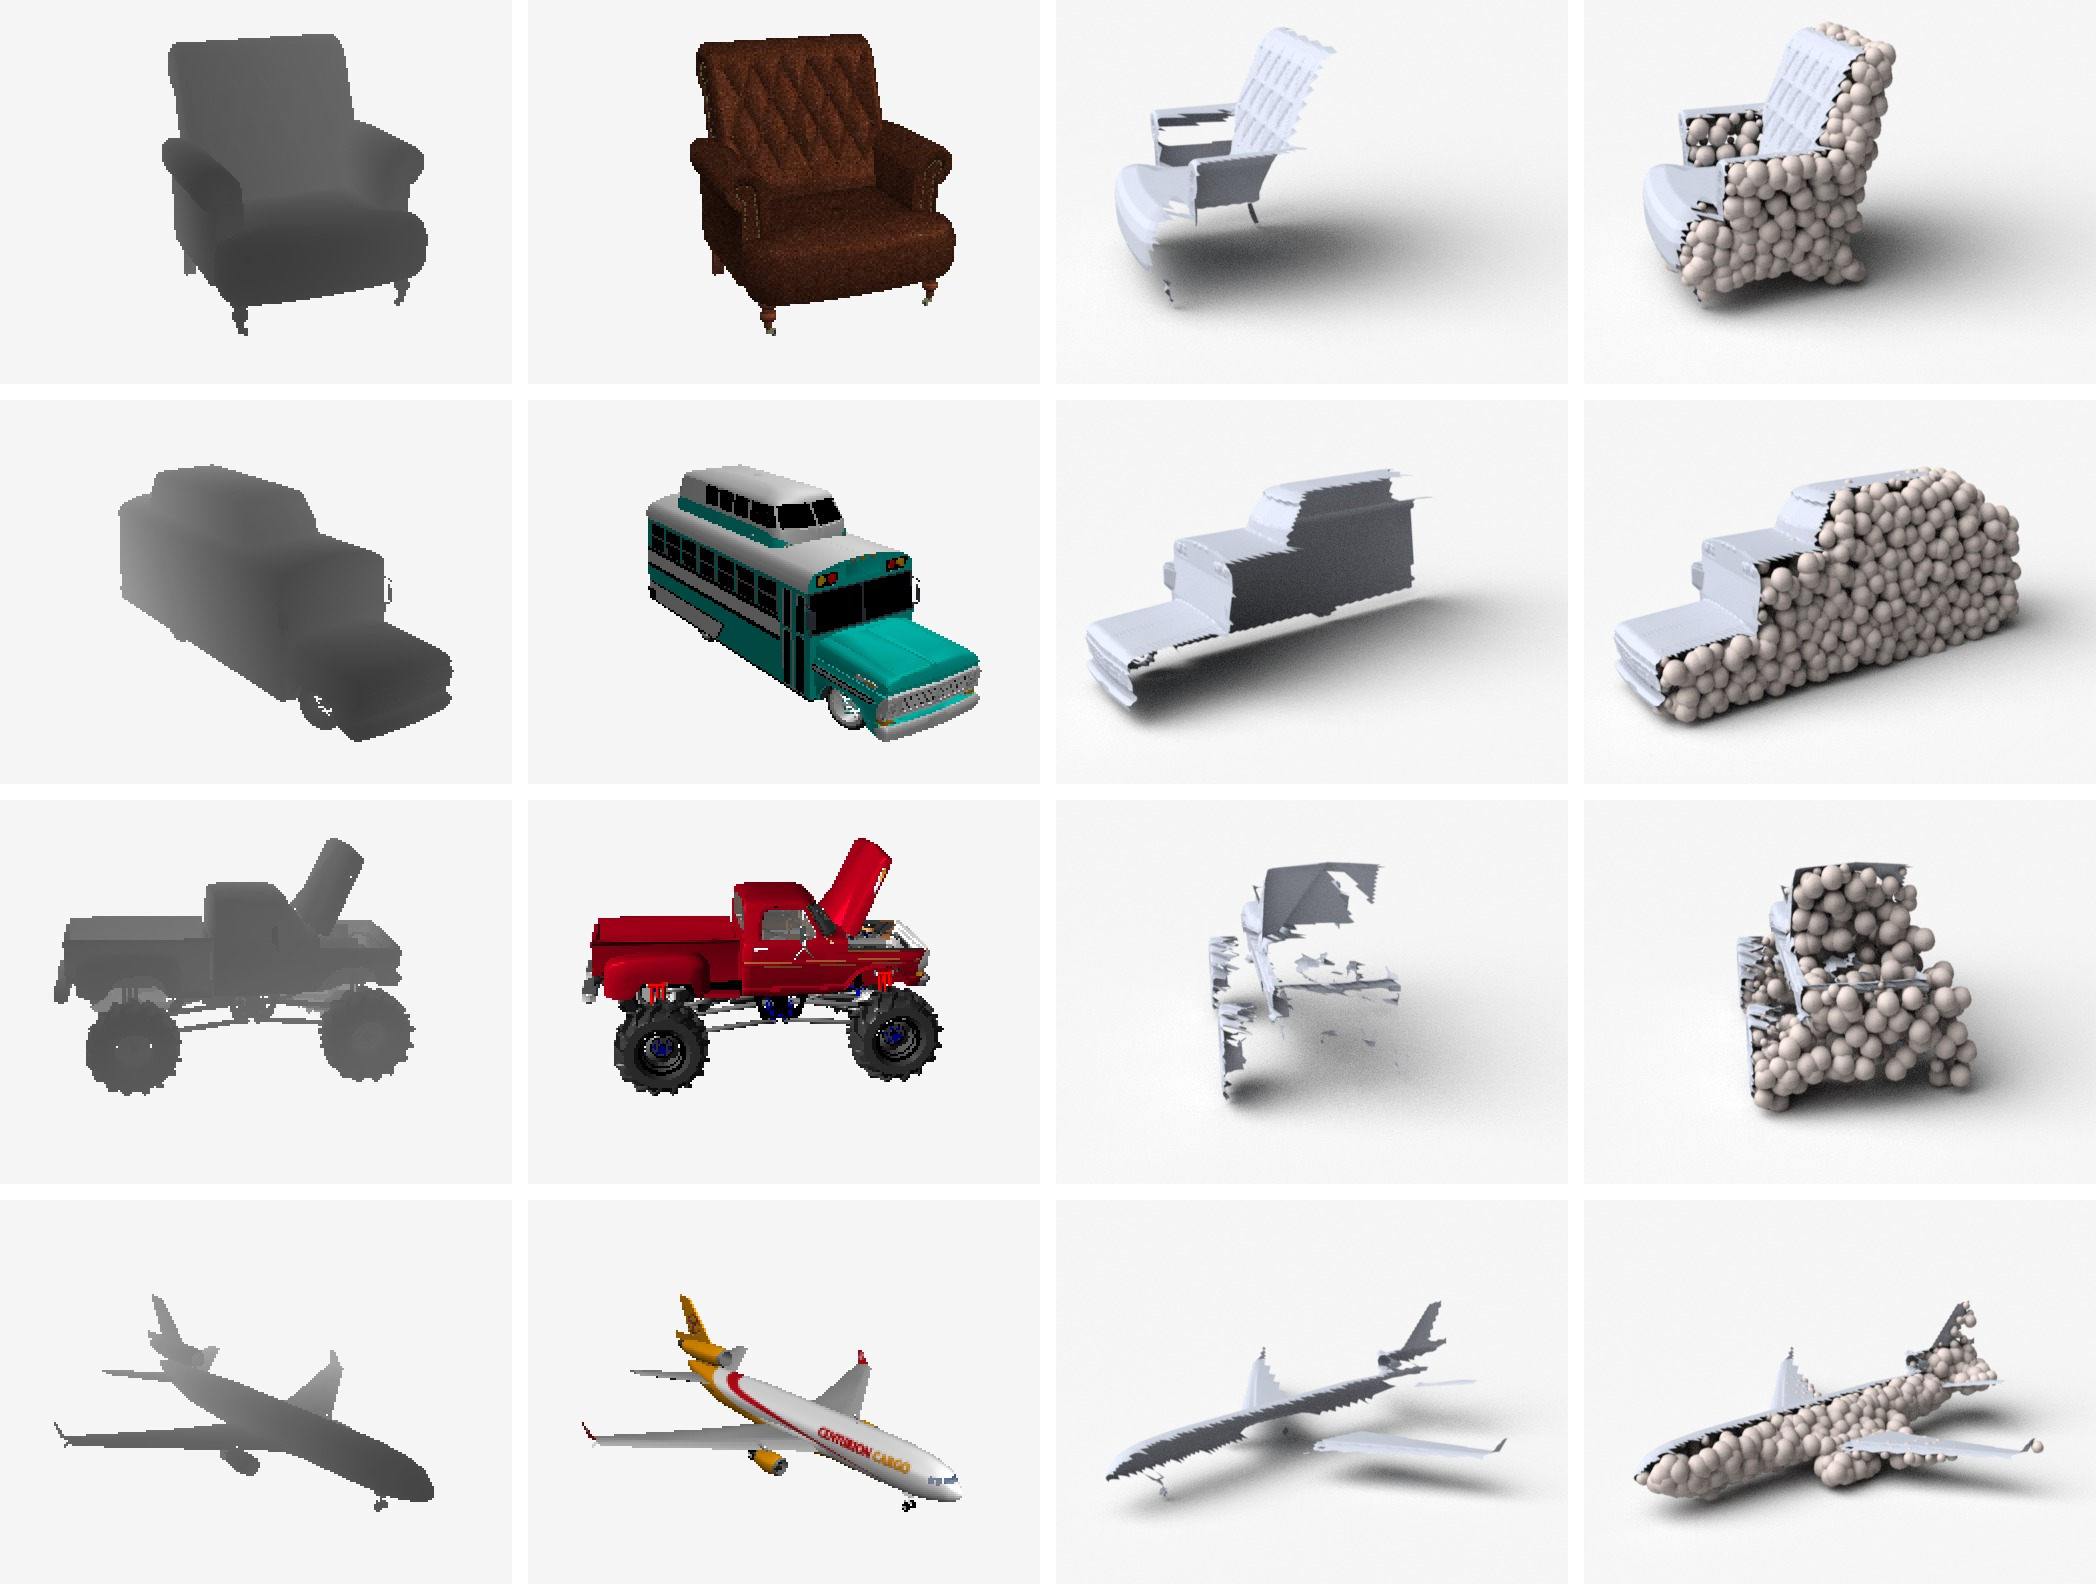
\includegraphics[width=0.9\linewidth]{./fig/completion}
  \caption{Shape completion from a single RGBD image.}\label{fig:shape_completion}
\end{figure}
One interesting feature of our approach is that we can easily inject additional input information into the system. When the neural network is given RGBD input our system can be viewed as a 3D shape completion method. Fig~\ref{fig:shape_completion} visualizes examples of the predictions.

The neural network successfully guesses the missing parts of the model. By using the shape priors embedded in the object repository, the system can leverage cues of both symmetry (e.g. airplanes should have symetric sides) and functionality (tractors should have wheels). The flexible representation of point set facilitates the resolution of the object's general shape and topology. More fine-grained methods that directly exploit local geometric cues could be cascaded after our predictions to enrich higher frequency details.

\subsection{Predicting Multiple Plausible Shapes}
\label{sec:exp:gan}
\begin{figure}[t!]
  \centering
  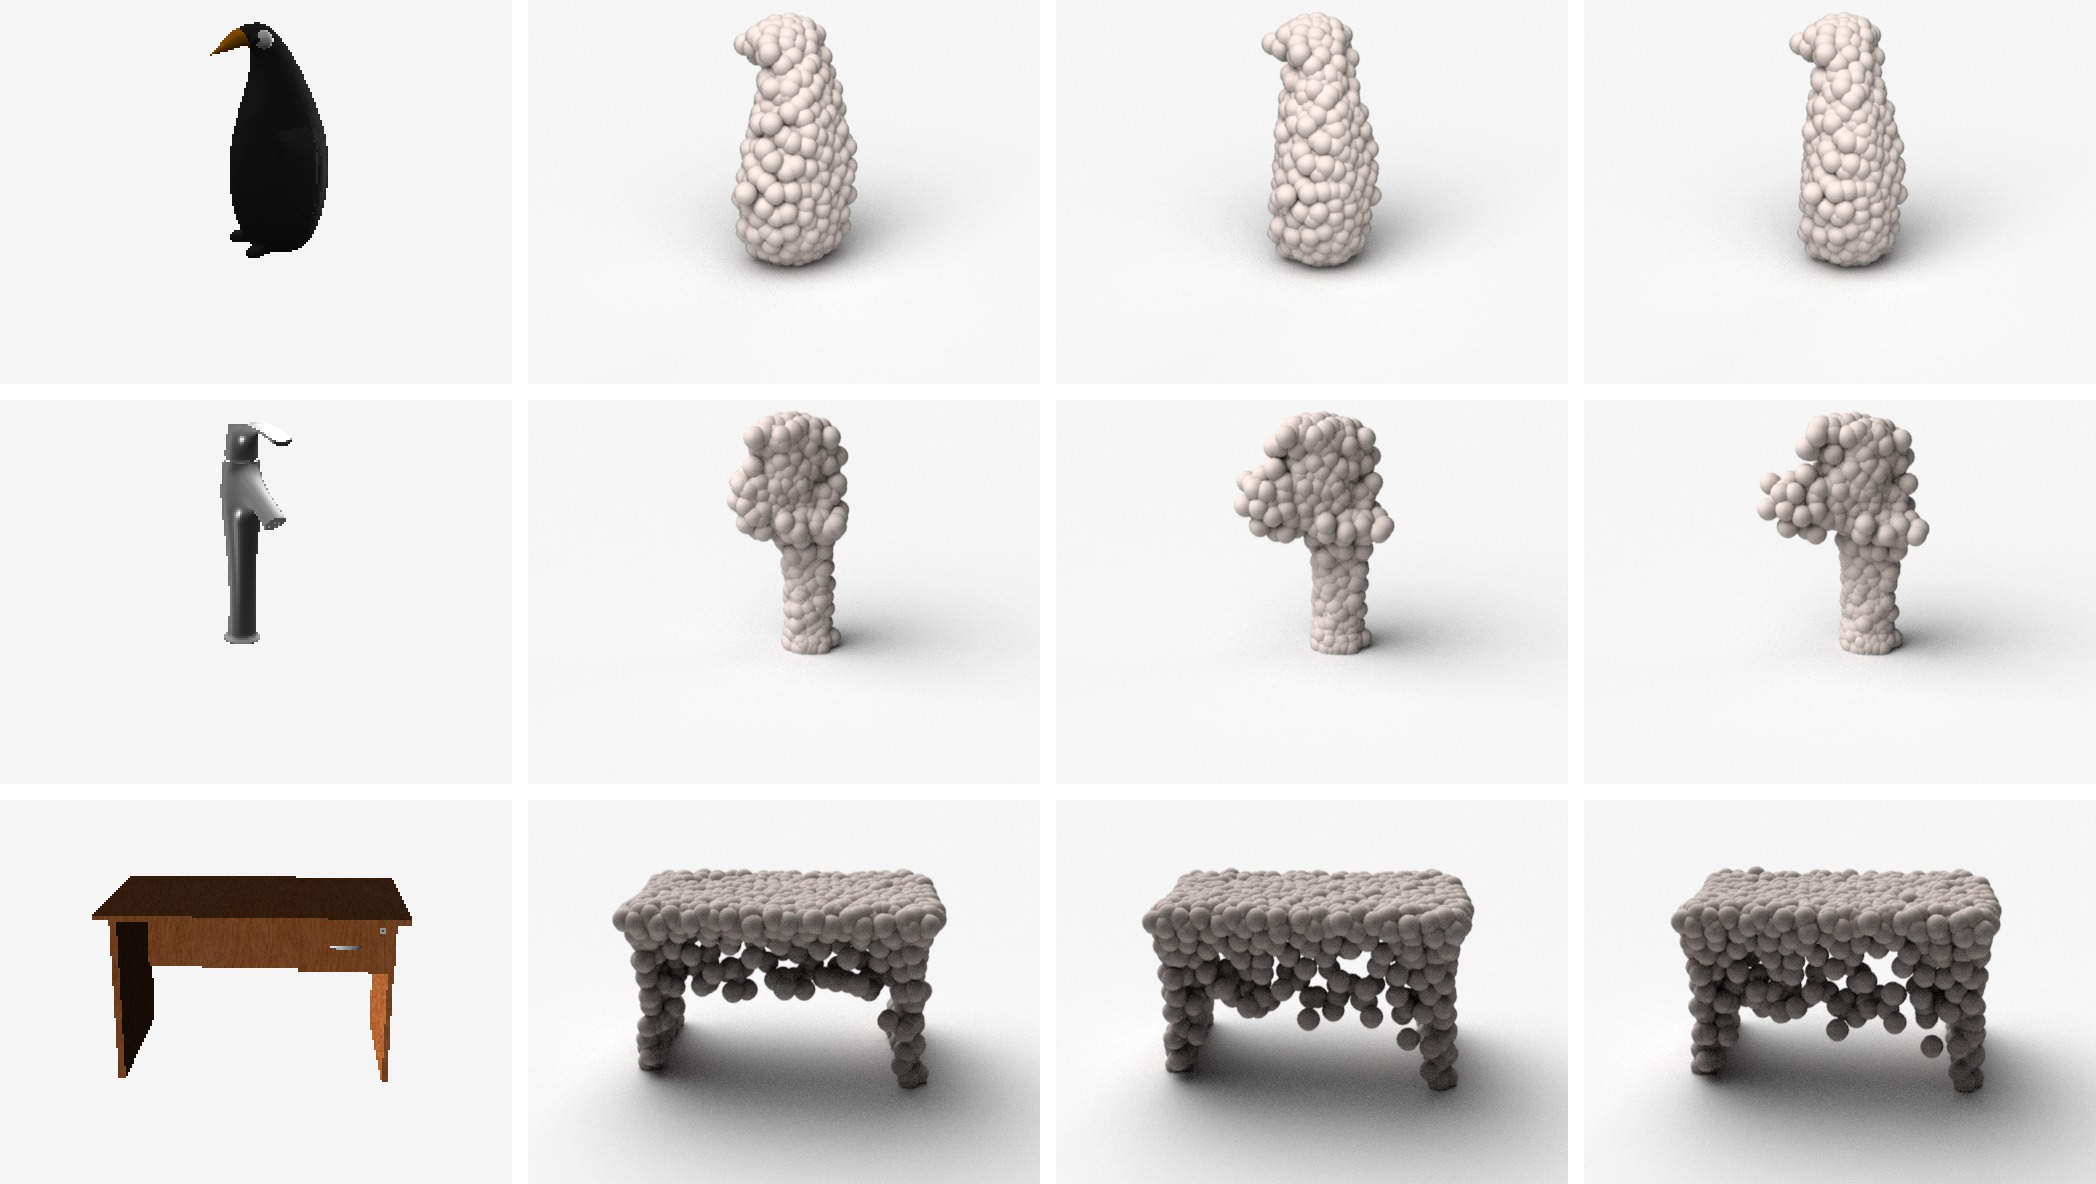
\includegraphics[width=0.9\linewidth]{./fig/ambiguity}
  \caption{Multiple predictions for a single input image. The point sets are visualized from different view points (top row: half side view, middle row: side view, bottom row: back view) to better reveal the difference.}\label{fig:deformation}
\end{figure}

\begin{figure}
\centering
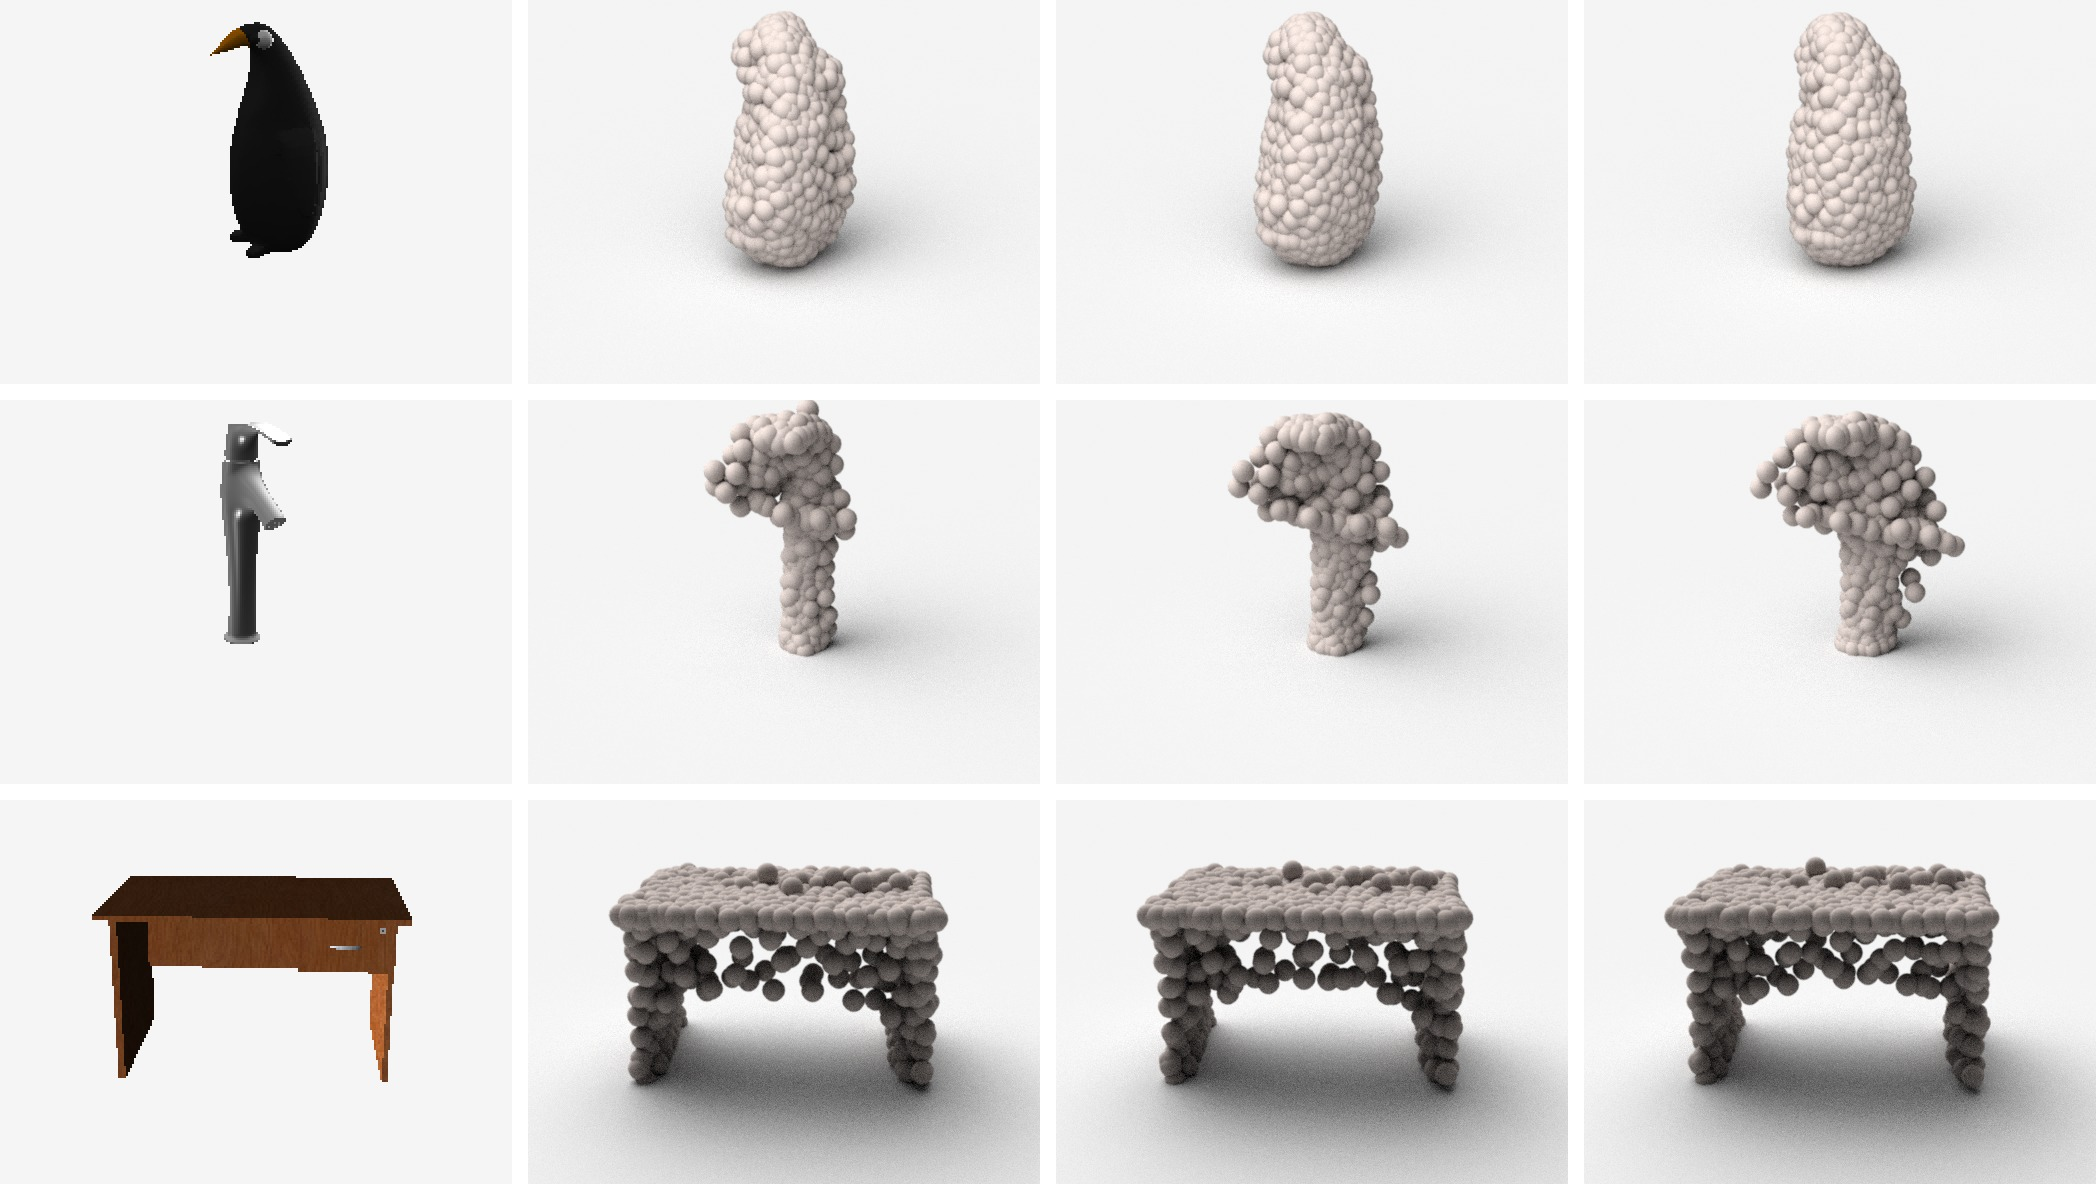
\includegraphics[width=0.9\linewidth]{./fig/show_vae}
\caption{Result obtained by VAE training. Top: half-side view; middle: side view; bottom: back view.}
\label{fig:show_vae}
\end{figure}

The randomness in our network enables prediction of different shapes given the same input image. To show this, we take the RGB image as the input. During training we handle randomness by using either the Mo2 or the VAE method. At test time when the ground truth is unknown, the random numbers are sampled from the predefined distribution.

Fig~\ref{fig:deformation} plots examples of the set of predictions of our method. The network is able to reveal its uncertainty about the shape or the ambiguity in the input. Points that the neural network is certain about its position moves little between different predictions. Along the direction of ambiguity (e.g. the thickness of the penguin's body) the variation is significantly larger. In this figure we trained our network with Mo2 and Chamfer Distance. In Fig~\ref{fig:show_vae}, we visualize the results of VAE. Compared to the result of Mo2, the prediction of VAE looks plumper; however, it also captures the local directions of ambiguity in the shape.

\begin{figure}[h!]
  \centering
  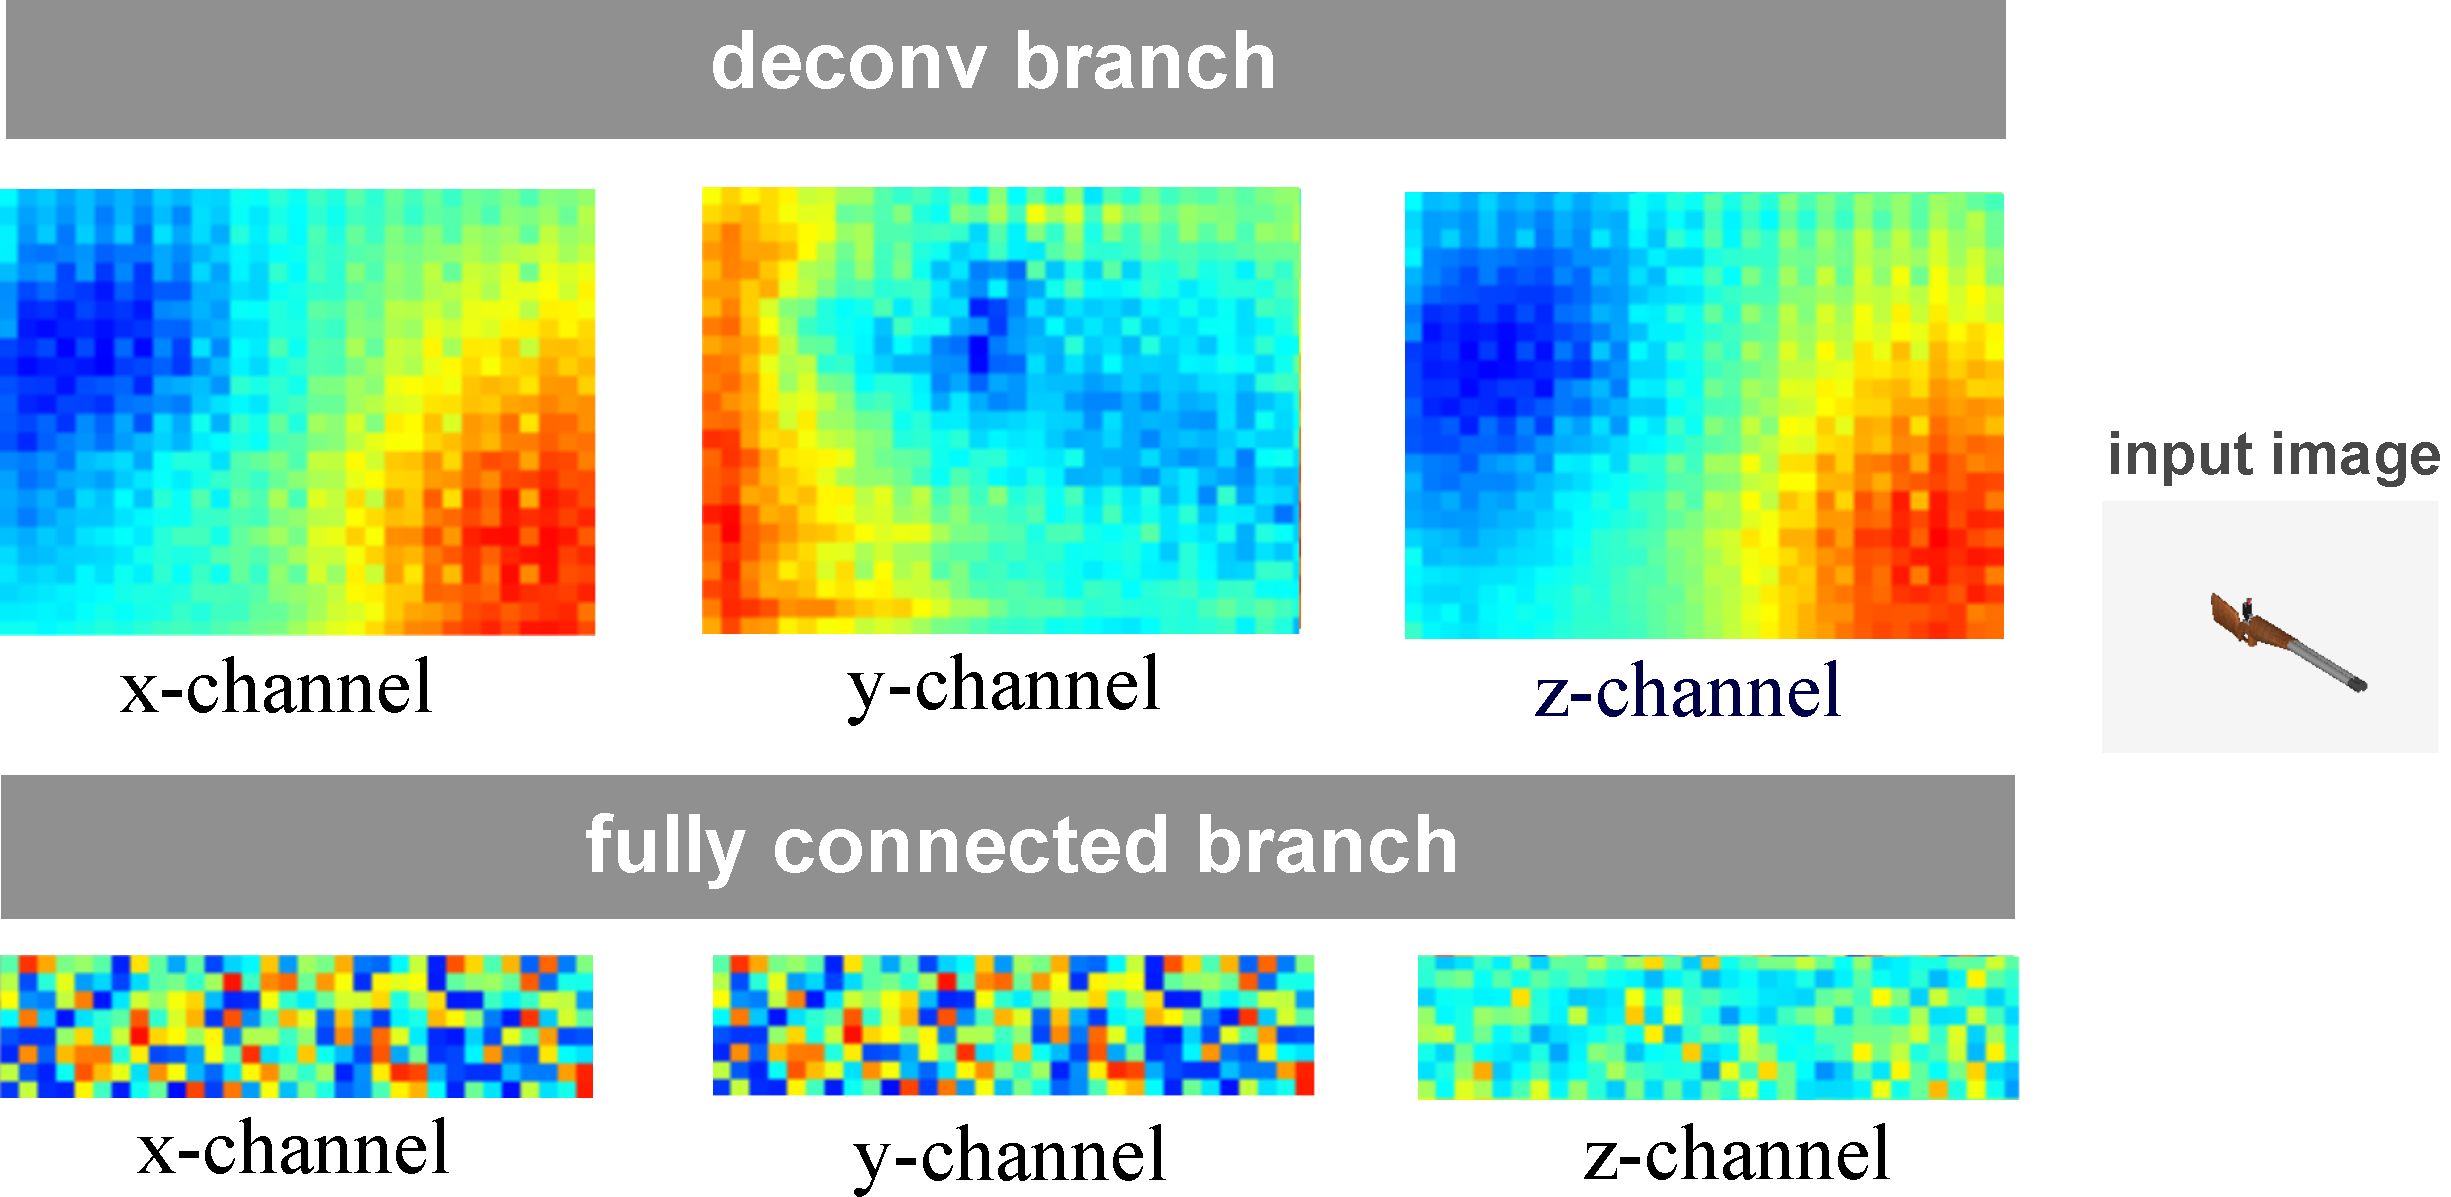
\includegraphics[width=0.9\linewidth]{./fig/show_channels}
  \caption{Visualization of the channels.}\label{fig:vis_deconv_channels}
  \vspace{-1em}
\end{figure}
\subsection{Network Design Analysis}



\begin{figure}[!]
  \centering
  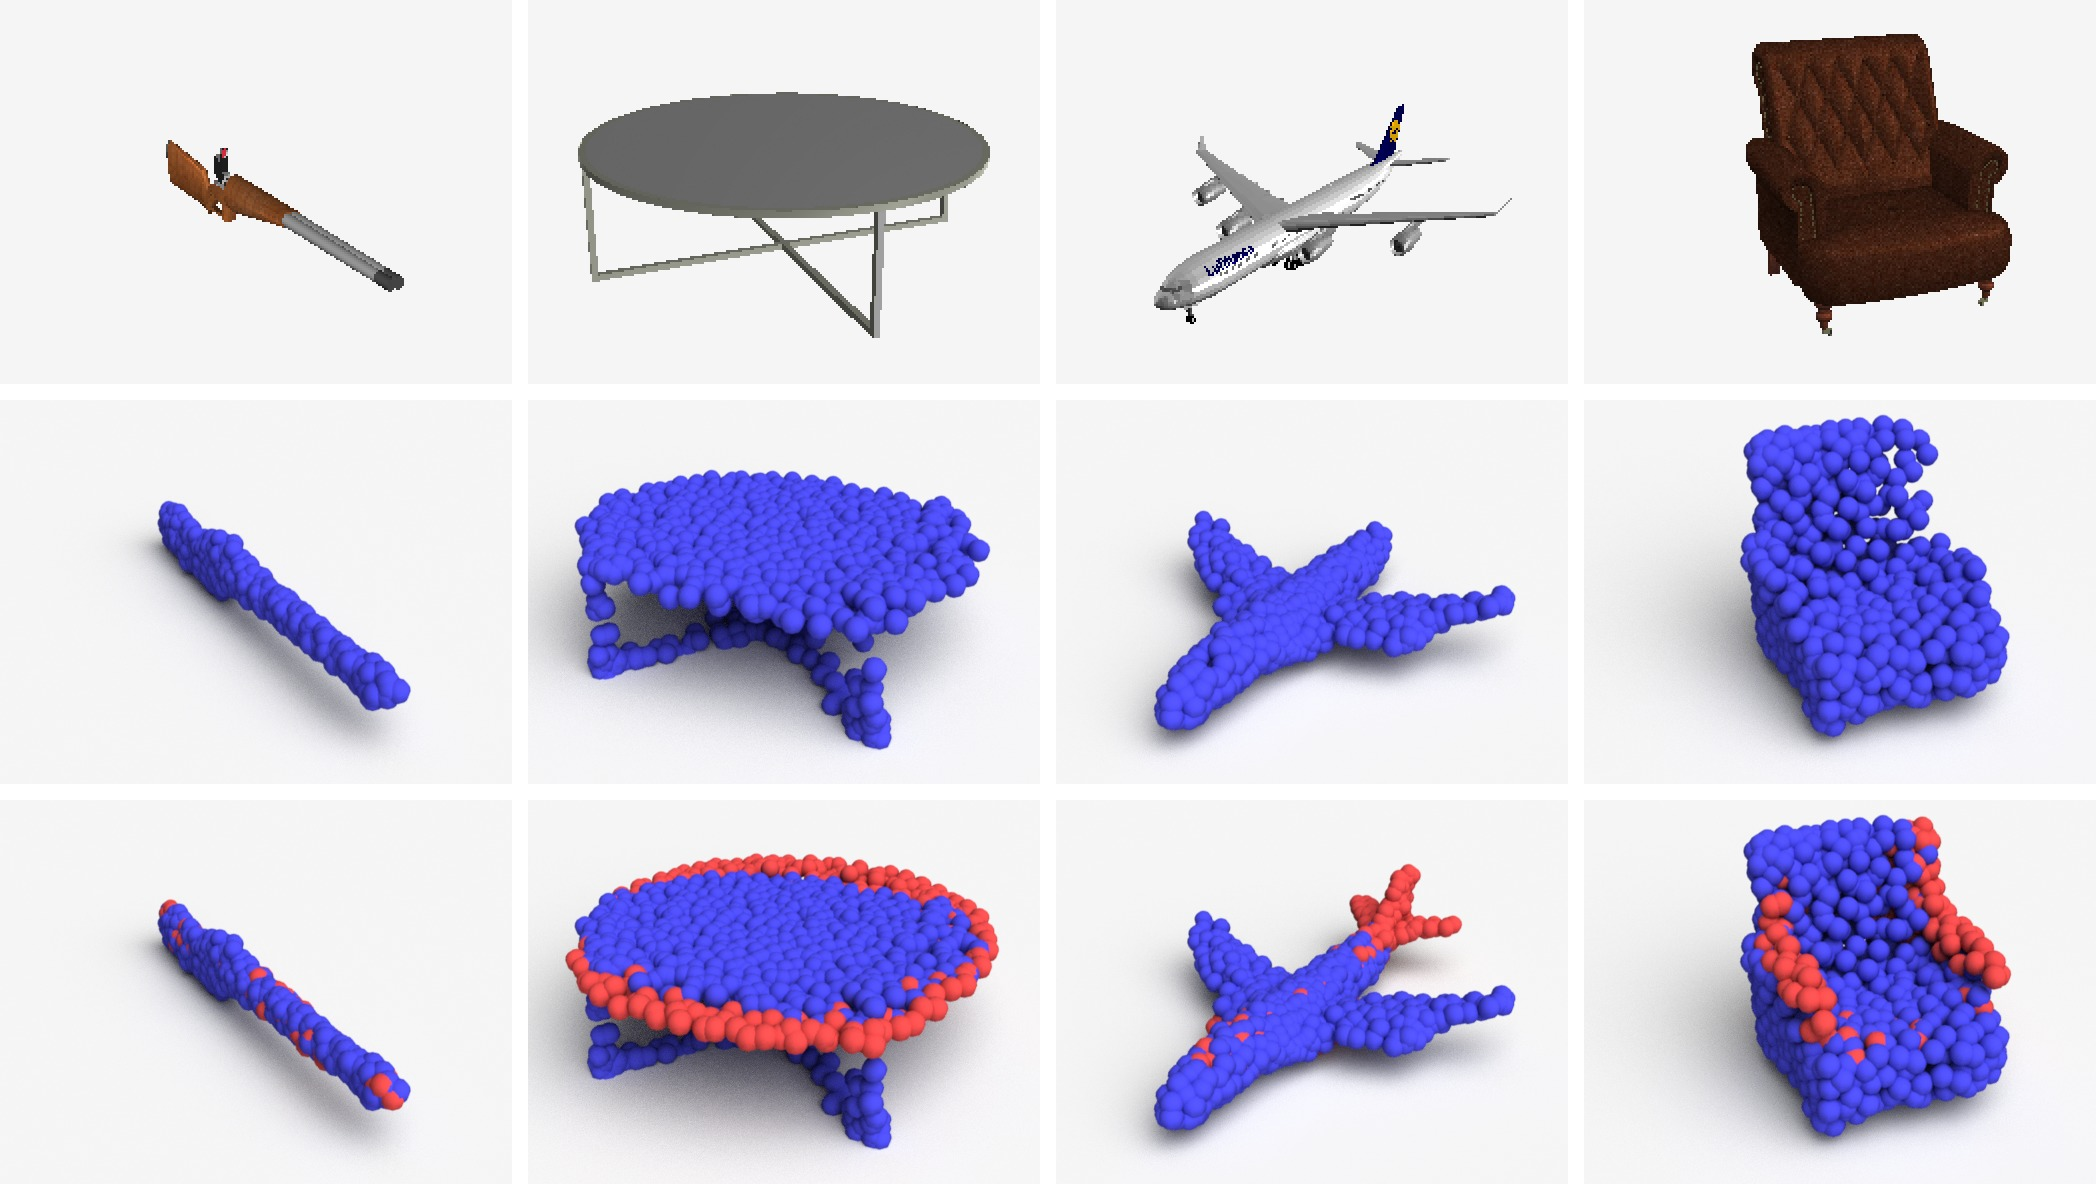
\includegraphics[width=0.9\linewidth]{./fig/two_branch}
  \caption{Visualization of points predicted by the deconvolution branch (blue) versus the fully connected branch (red).}\label{fig:vis_deconv_vs_fc}
  \vspace{-1em}
\end{figure}
\label{sec:exp:analysis}
\paragraph{Effect of combining deconv and fc branches for reconstruction}

\begin{figure*}[t!]
   \centering
   \vspace{1em}
   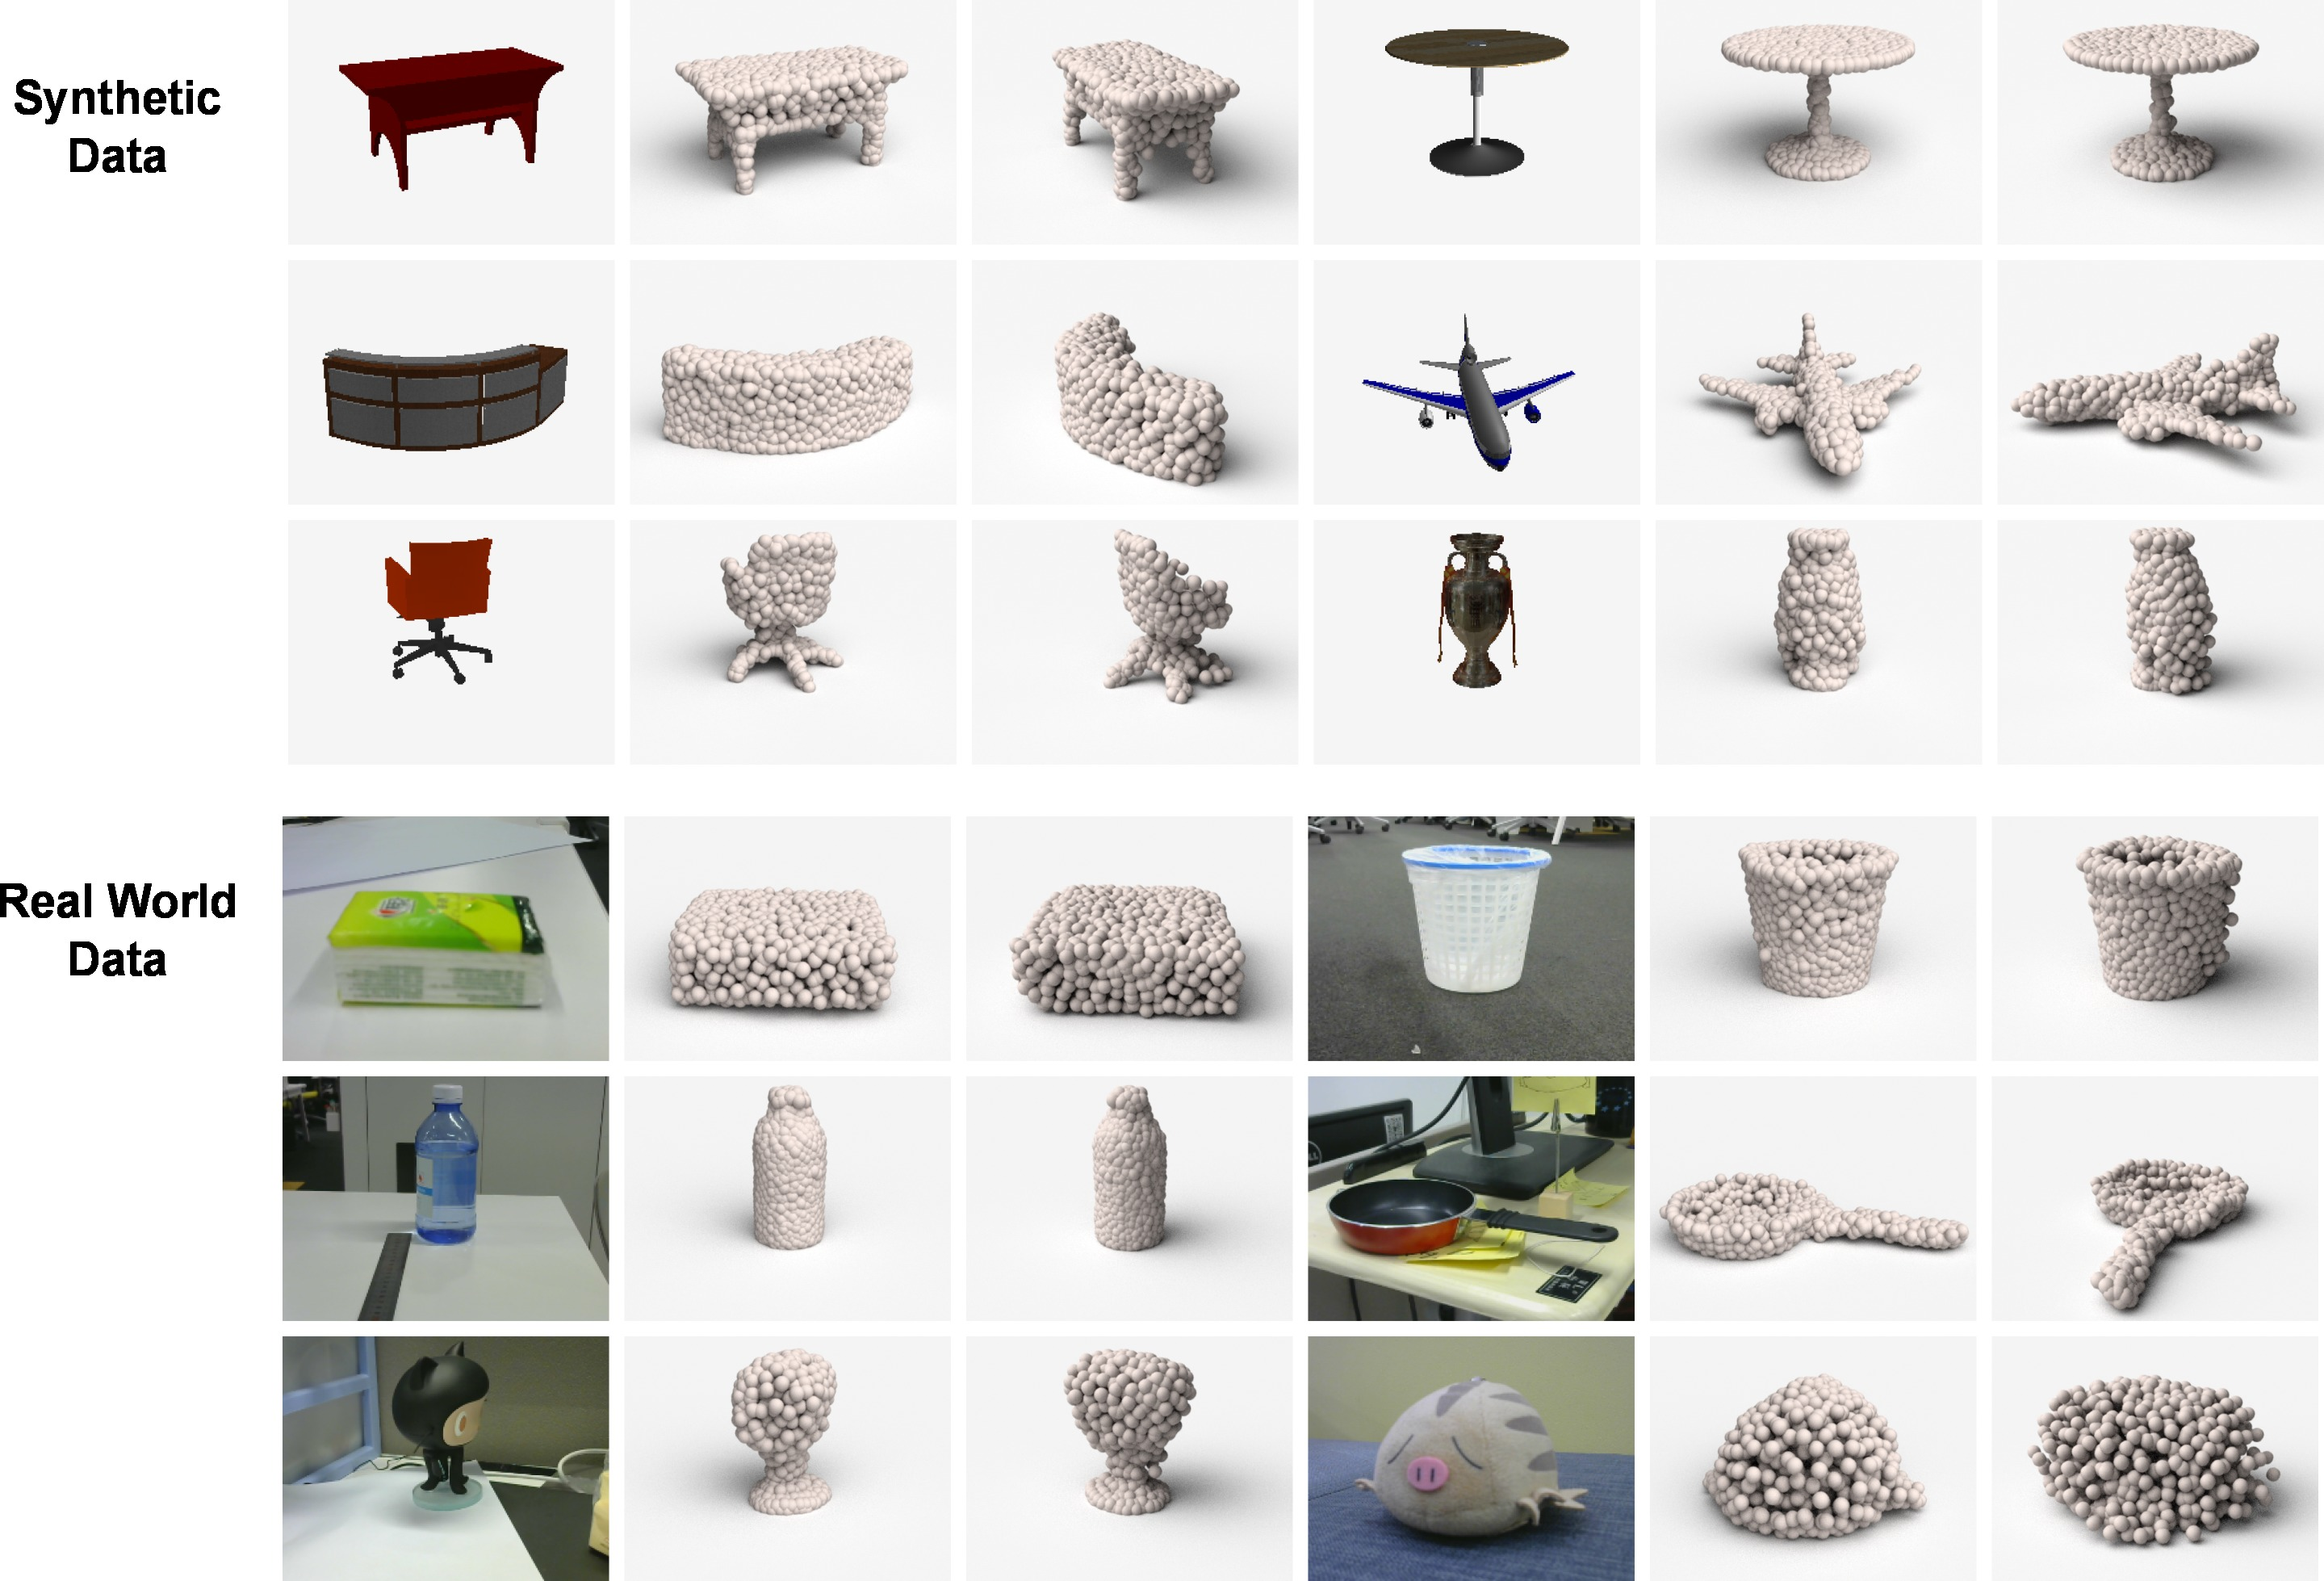
\includegraphics[width=0.9\linewidth]{./fig/realworld}
   \caption{Visualization of predictions on synthetic and real world data.}\label{fig:more_examples}
 \end{figure*}
We compared different designs of the neural network architectures. The performance values are reported based on our own rendered training set.% in the studio setup. 
As shown in Fig~\ref{fig:compare_networks}, the introduction of deconvolution significantly improves performance. Stacking another hourglass level also gives performance gain.

\begin{figure}[t!]
  \centering
  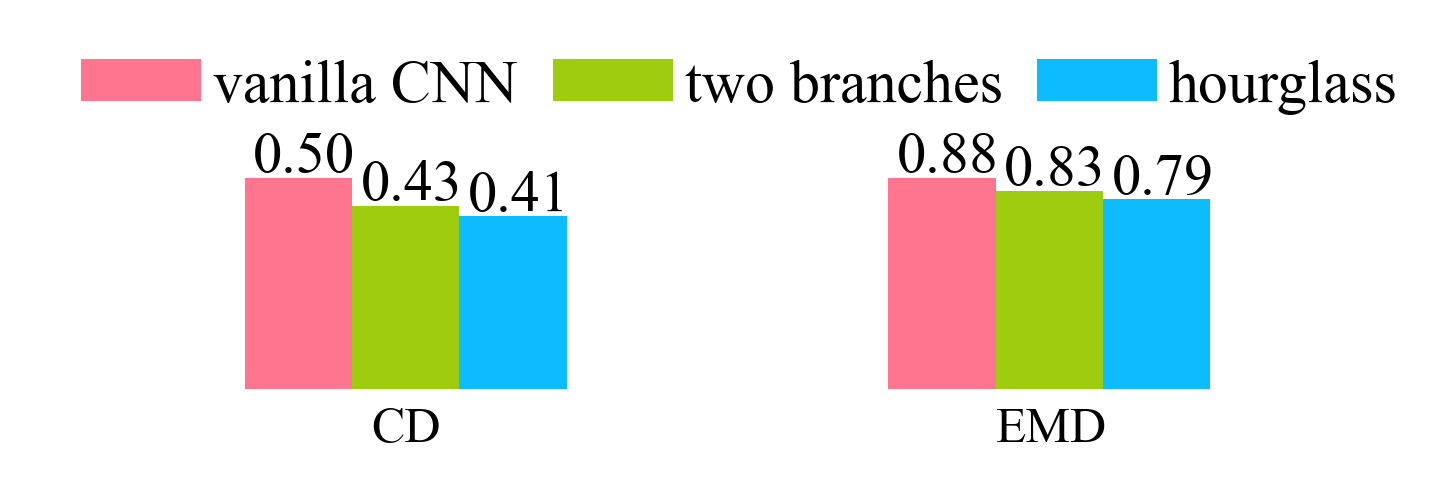
\includegraphics[width=\linewidth]{./fig/network_bar}
  \caption{Comparison of different networks by Chamfer Distance (CD) and Earth Mover Distance (EMD). More complex network gives slightly better results. }\label{fig:compare_networks}
  \vspace{-1em}
\end{figure}

We further visualize the output of the deconv branch and fully connected branch separately to gain a better understanding of their functions. In Fig~\ref{fig:vis_deconv_channels} the values in the x, y and z channels are plotted as 2D images for one of the models. In the deconv branch the network learns to use the convolution structure to constructs a 2D surface that warps around the object. In the fully connected branch the output is less organized as the channels are not ordered.


In Fig~\ref{fig:vis_deconv_vs_fc} we render the two set of predictions in 3D space. The deconv branch is in general good at capturing the ``main body'' of the object, while the fully connected branch complements the shape with more detailed components (e.g. tip of gun, tail of plane, arms of a sofa). This reveals the complementarity of the two branches. The predefined weights sharing and node connectivity endow the deconv branch with higher efficiency when they are congruent with the desired output's structure. The fully connected branch is more flexible but the independent control of each point consumes more network capacity.


% \paragraph{Choice of point set distance}
% We compare the results obtained by minimizing the Chamfer distance and earth mover distance.
% Fig~\ref{fig:choice_of_point_set_distance} visualizes the effect of alternative point set distance metrics on synthetic data.

\paragraph{Analysis of distance metrics}

Different choices of the loss functions have distinct effect on the network's prediction pattern. Fig~\ref{fig:emd_vs_chamfer} exemplifies the difference between two networks trained by CD and EMD correspondingly. The network trained by CD tends to scatter a few points in its uncertain area (e.g. behind the door) but is able to better preserve the detailed shape of the grip. In contrast, the network trained by EMD produces more compact results but sometimes overly shrinks local structures. This is in line with experiment on synthetic data.

\begin{figure}[ht!]
  \centering
  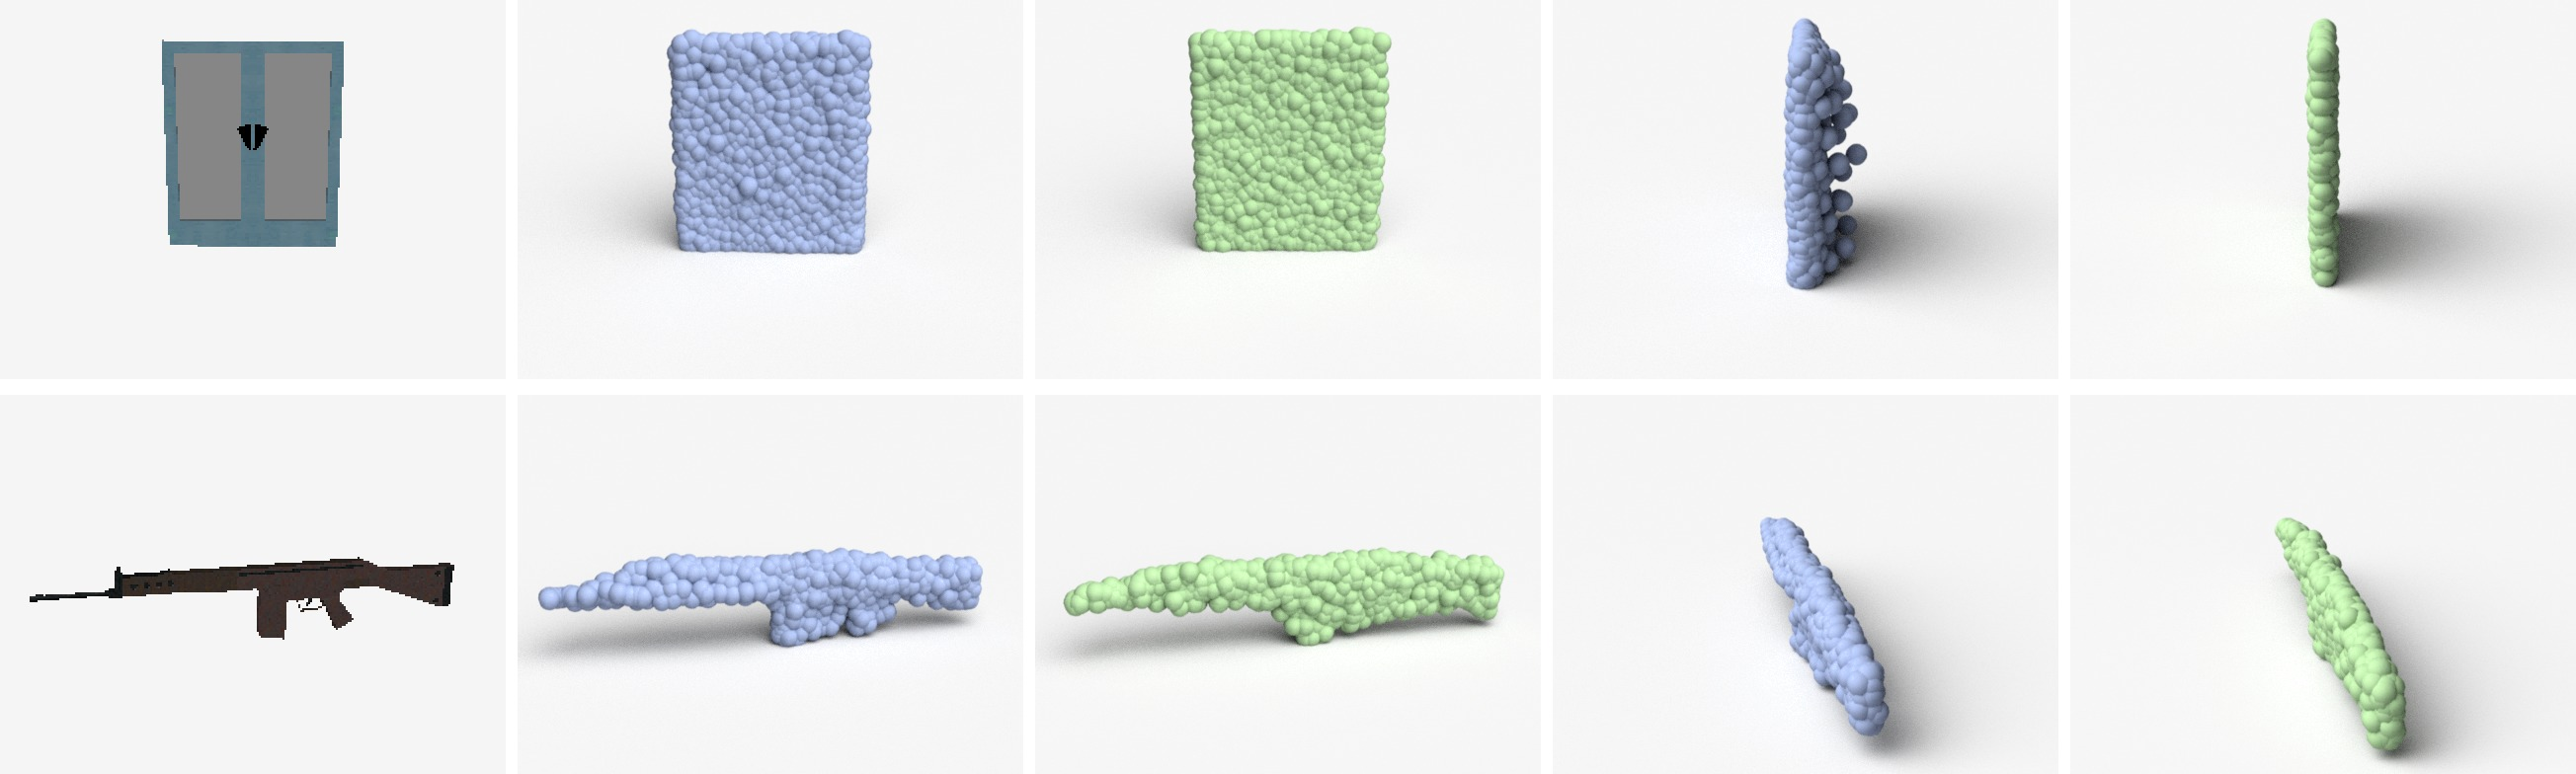
\includegraphics[width=\linewidth]{./fig/show_emd_vs_chamfer}
  \caption{Comparison of predictions of networks trained by CD (blue, on the left) and EMD (green, on the right). }\label{fig:emd_vs_chamfer}
  \vspace{-1em}
\end{figure}

\subsection{More results and application to real world data}
\label{sec:exp:more}
 
Fig~\ref{fig:more_examples} lists more example predictions on both synthetic data and real world photos. For real world photo, we mask out background pixels to indicate the object. Our algorithm gives promising result though trained on synthetic data only.
We plot the reconstruction results of the first 5 mini-batches (160 cases in total) of our validation set at the end of this paper in Fig~\ref{fig:show_all}. Results produced by the network trained by CD and EMD are compared side-by-side. Owing to the diversity in the ShapeNet dataset, our system is able to handle a variety of object types.



\subsection{Analysis of human ability for single view 3D reconstruction}
We conducted human study to provide reference to our current CD and EMD values reported on the rendered dataset. We provided the human subject with a GUI tool to create a triangular mesh from the image. The tool (see Fig~\ref{fig:gui_tool}) enables the user to edit the mesh in 3D and to align the modeled object back to the input image. In total 16 models are created from the input images of our validation set. $N=1024$ points are sampled from each model.

\begin{figure}
\centering
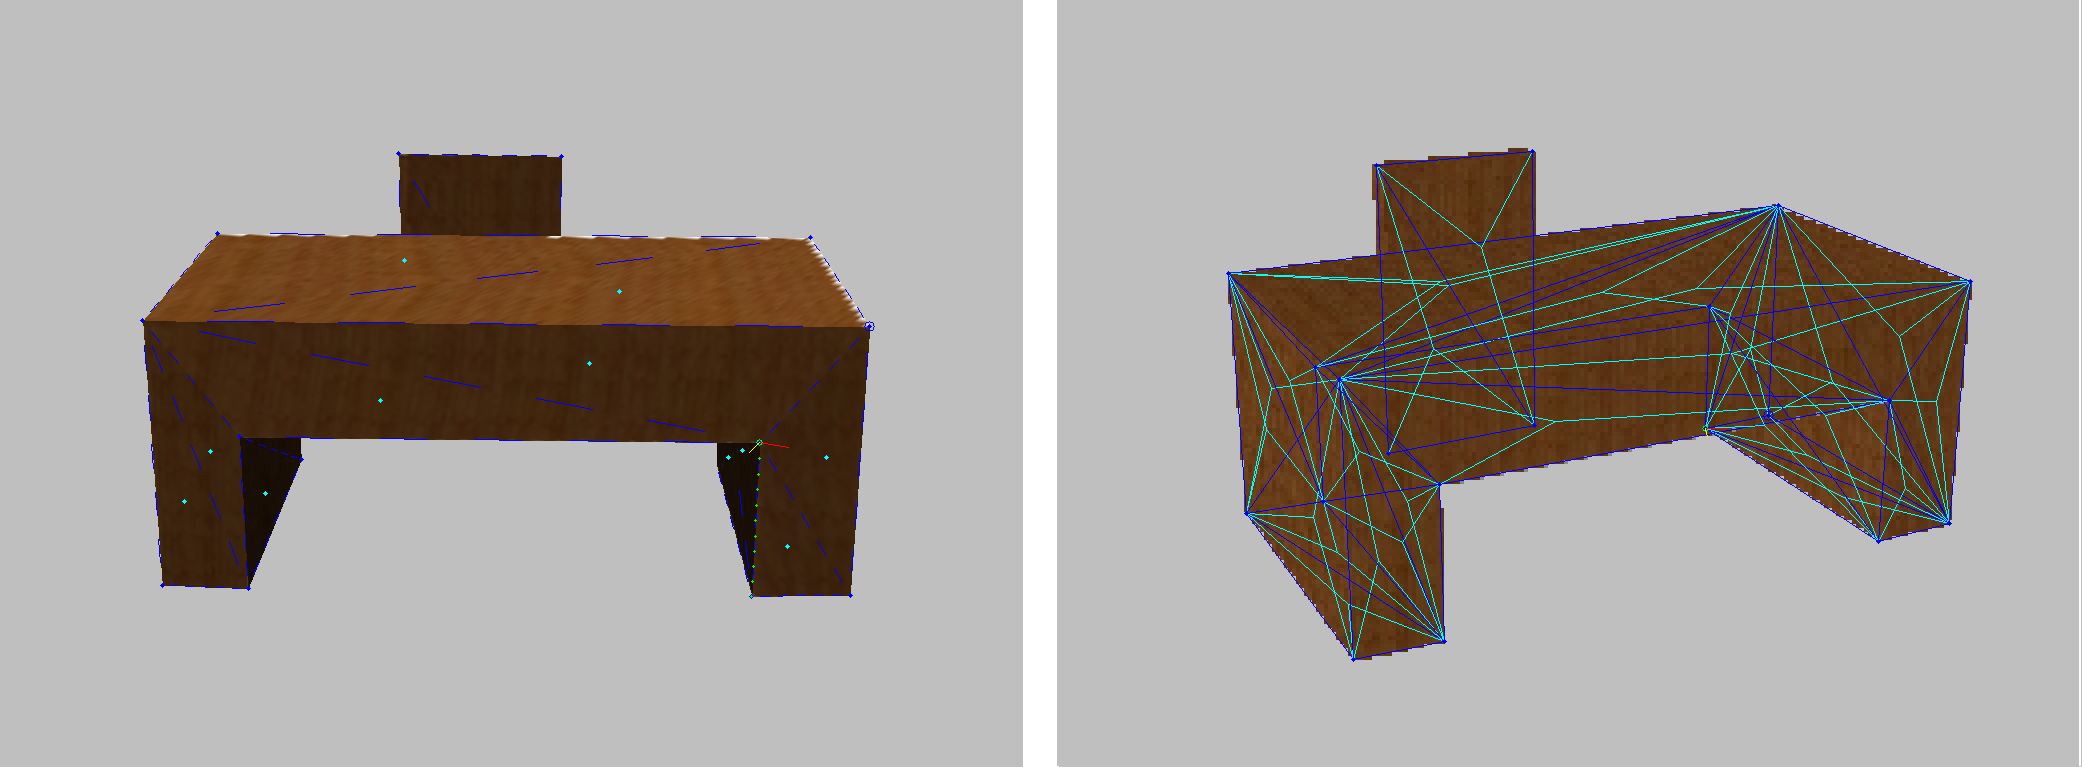
\includegraphics[width=1.0\linewidth]{./fig/label_tool}
\caption{GUI tool used to manually model the objects. The user can change view point, edit vertex positions and connectivity in the 3D view (bottom). We also overlaid a wire-frame rendering of the object on the input image (top) to facilitate alignment.}
\label{fig:gui_tool}
\end{figure}

\begin{figure}
\centering
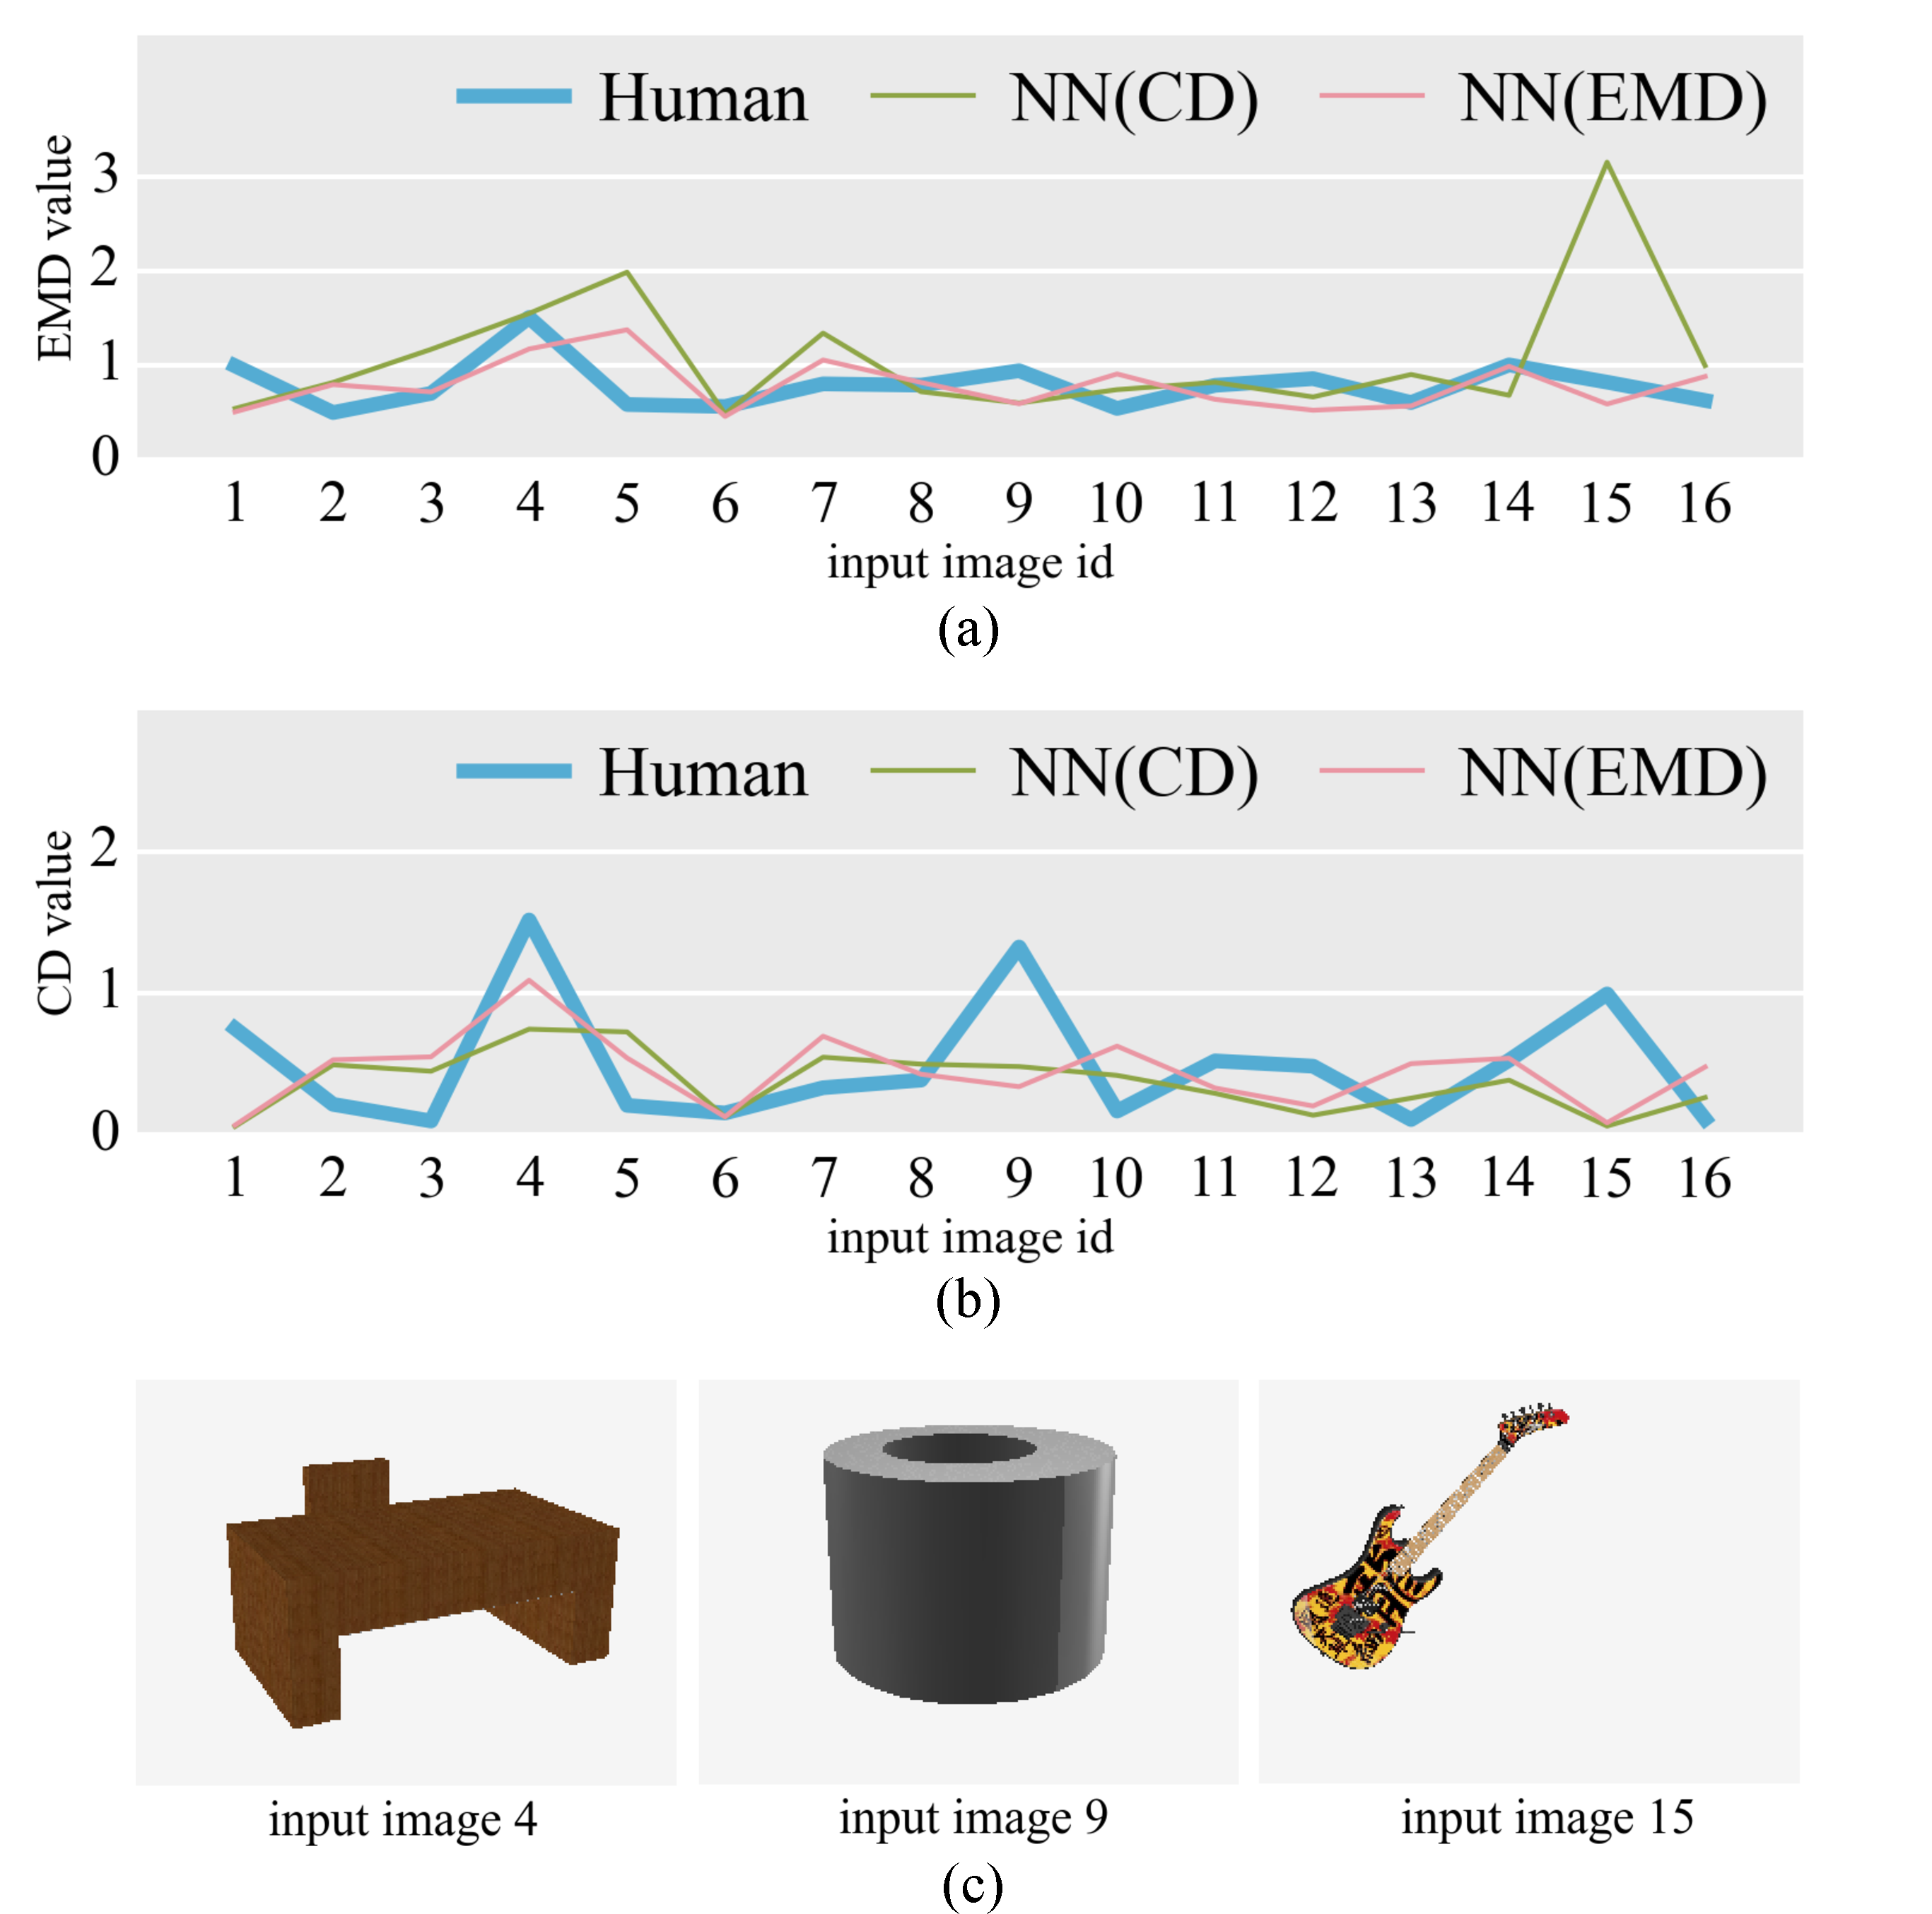
\includegraphics[width=1.0\linewidth]{./fig/show_human}
\caption{Comparison of reconstructions generated by the human subject, the neural network trained with CD and the neural netword trained with EMD on 16 input images in the validation set. (a) Comparison of EMD value. (b) Comparison of CD value. (c) Input images numbered 4, 9 and 19 on which the human subject performs poorly.}
\label{fig:human_number}
\end{figure}

As shown in Fig~\ref{fig:human_number}, both the EMD and the CD values of the network's reconstruction are on par with human's manual creation for most of the cases. We observed that the human subject mainly used cues of gravity direction (legs of chairs should touch the ground) and symmetry to infer the object's shape. As illustrated in input image number 4, 9 and 15, when the object is partially occluded (the table blocks the chair), ambiguous (it is unclear whether the can has a bottom) or manifests inadequate geometric cues (the guitar has non-polygonal shape and does not sit on the ground) the human subject performs poorly. The neural network trained by EMD performs reasonably well under both metrics. However, because CD emphasises only on the best matching point, the network trained by CD does not always produce predictions of uniform density and suffers high EMD value in some cases.

\subsection{Analysis of failure cases}
%\todo{
%\begin{itemize}
    %\item shape completion numbers    
    %\item shape reconstruction examples (point cloud as %.pcd file)
    %\item shape completion examples (point cloud as .pcd %file)
    %\item a video
%\end{itemize}
%}

\begin{figure}
\centering
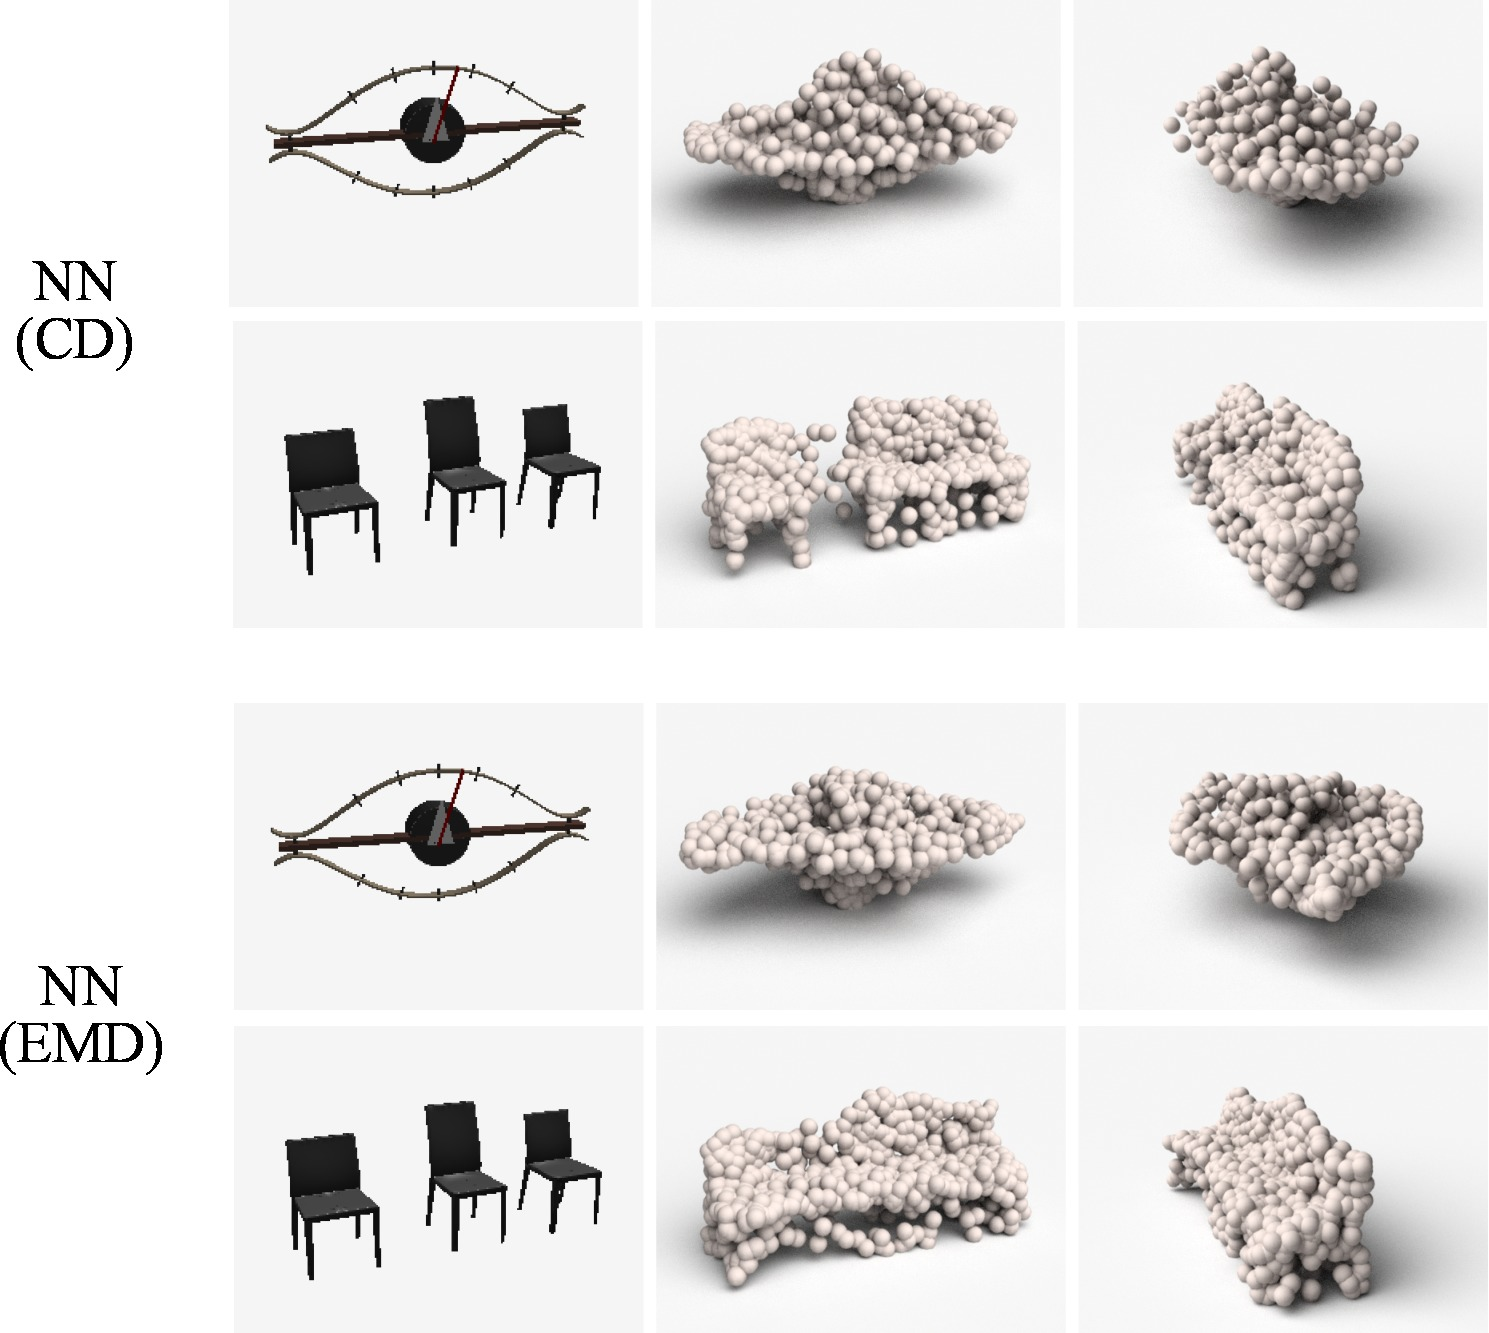
\includegraphics[width=\linewidth]{./fig/show_failure}
\caption{Examples of failure cases of our method on the validation set. Top: results of the neural network trained by CD. Bottom: results of the neural network trained by EMD. Both networks give unsatisfactory results.}
\label{fig:failure_case}
\end{figure}

We visualize representative failure cases of our method on our rendered validation set. There are two trends, each exemplified by one input case in Fig~\ref{fig:failure_case}. In the first kind of failure cases, the neural network is presented with a shape that it has completely no idea about. Then the networks tried to explain the input by something similar (a plane without wings?) but fundamentally wrong. In the second kind of failure cases, the neural network sees a composition of multiple objects. Because we have not implemented any detection or attention mechanism, the networks produce distorted output.


\subsection{Implementation details}
\label{sec:impl_details}
\paragraph{Network parameter and training}
Our network works on input images of 192x256. The deconv branch produces 768 points, which correspond to a 32x24 three-channel image. The fully connected branch produces 256 points. The convolutional layer has 16 feature maps in the highest resolution, and the number of channels are doubled after each decrease in resolution. We use strided convolution instead of max-pooling to increase speed. The training program is implemented in TensorFlow. 300000 gradient steps are taken, each computed from a minibatch of 32. Adam is used as the optimizer. We observed that the training procedure is smooth even without batch normalization. All activation functions are relu.

\paragraph{Post processing}
We use a local method to post process the point cloud into a volumetric representation. First, the point cloud is registered into the 32x32x32 grid with bilinear interpolation. This can be think of as interpreting the points as 1x1x1 cubes and averaging the intersection volume with each grid cell (the occupancy representation). Then each voxel exams a local neighborhood to determine the final value. We implement this as a trained 3D convolutinoal neural network with 6 layers of 3x3x3 convolutions. This post-processing network is trained by IoU on the same training partition as the point cloud generation network. In order to compensate for difference in point density among objects of different volumes, we trained another network to predict the object's volume. The predicted volume is concatenated with the registered occupancy as the 3D conv network's input. Using the point cloud generation network trained by either EMD or CD to is enough to outperform 3D-R2N2's result. The maximum performance as reported in the main paper is obtained by feeding both     network's prediction into the post processing network. We also notice that the volume prediction network is not necessary to outperform 3D-R2N2. However, it consistently gives performance gain, so we kept this component in our experiments.
